\begin{sidewaysfigure}
\centering
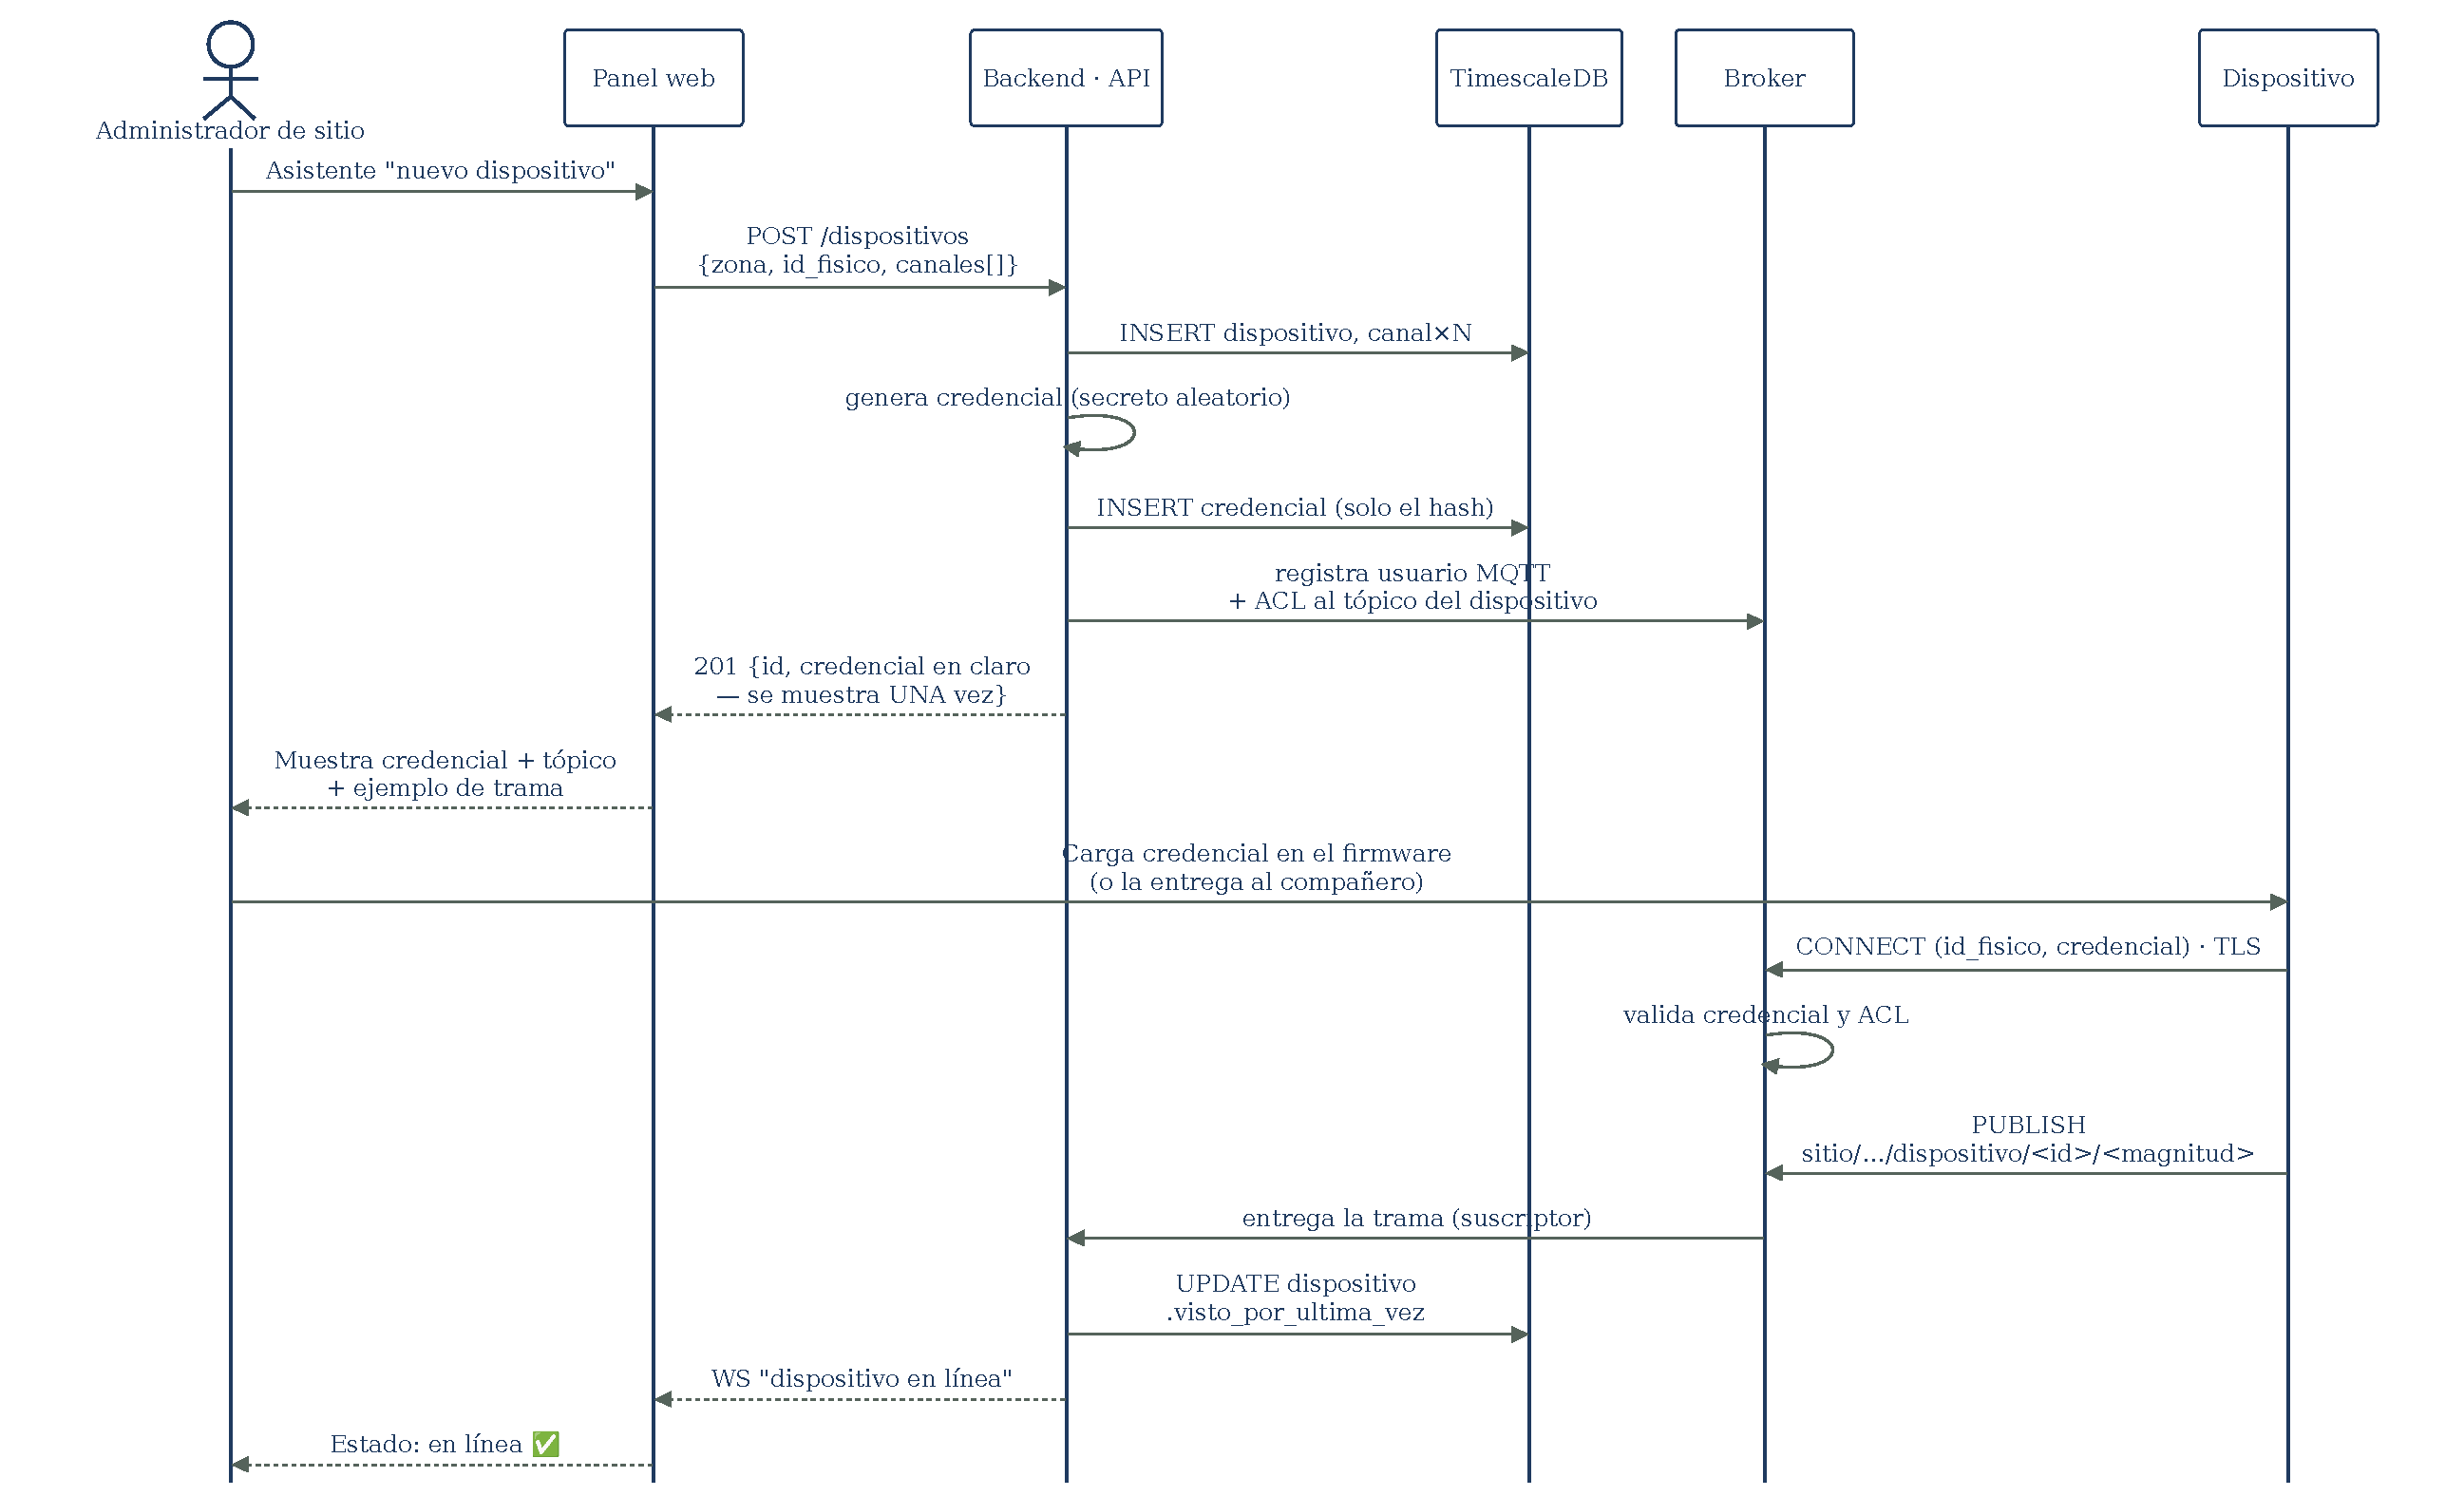
\includegraphics[width=0.96\textheight,height=0.9\textwidth,keepaspectratio]{figuras/render/sec-alta.pdf}
\caption{Aprovisionamiento de un dispositivo (diagrama de secuencia UML). Según la vía declarada (MQTT, HTTP o LoRaWAN, que autentica su pasarela), la credencial se genera en el servidor, se muestra una sola vez y en la base queda solo su hash; la ACL del broker limita al dispositivo a su propio tópico. Es el flujo que ataca la causa C4: una persona sin perfil técnico da de alta un sensor desde el panel. La ruta \texttt{POST /dispositivos} está implementada (Etapa 3); el alta desde el panel es de la Etapa 4.}
\label{fig:sec-alta}
\end{sidewaysfigure}
